\documentclass[11pt,aspectratio=169]{beamer}

\usepackage{rcstalk}
\usetheme{rcstheme}

\usepackage{graphicx}
\usepackage{tikz}
\usetikzlibrary{calc,positioning,shapes,decorations.pathreplacing}

% the styles for short and long nodes
\tikzset{
short/.style={draw,rectangle,text height=3pt,text depth=13pt,
  text width=7pt,align=center,fill=gray!30, line width=1.5pt},
long/.style={short,text width=1.5cm}
}

% the short nodes \shnode{<label>}{<right of>}{<text>}
\def\shnode#1#2{%
  \node[short,right=of #1] (#2) {}}
%\rotatebox{270}{#3}}}

% the long nodes \lnode{<label>}{<right of>}
\def\lnode#1#2{%
  \node[long,right=of #1] (#2) {}}

\usepackage{bytefield}

\topic{Memory allocation}
\subtitle{Lecture 9: Memory Allocation}

\begin{document}

\maketitle

\section{Malloc and fragmentation}

\begin{slide}{Dynamic memory allocation}
\itms{
  \item Almost all software uses dynamic memory management
  \ittms{
    \item Eases development and improves functionality
    \ittms{
      \item Don't have to statically specify complex data structures
      \item Can have data grow as a function of input size
      \item Allows recursive procedures (stack growth)
    }
    \item Problem: can have a huge impact on performance
  }
  \item Today: how to implement it
  \ittms{
    \item Lecture based on
      \cref{readings/wilson.pdf}{[Wilson]}
  }
  \item Some interesting facts:
  \ittms{
    \item Two or three line code change can have huge, non-obvious impact on 
	how well allocator works
    \item Proven: impossible to construct an "always good" allocator
    \item Memory management still poorly understood
  }
}
\end{slide}

\begin{slide}{Why is it hard?}
\itms{
  \item Satisfy arbitrary set of allocation and free's.
  \item Easy without free: set a pointer to the beginning of some big
    chunk of memory (``heap'') and increment on each allocation: \\
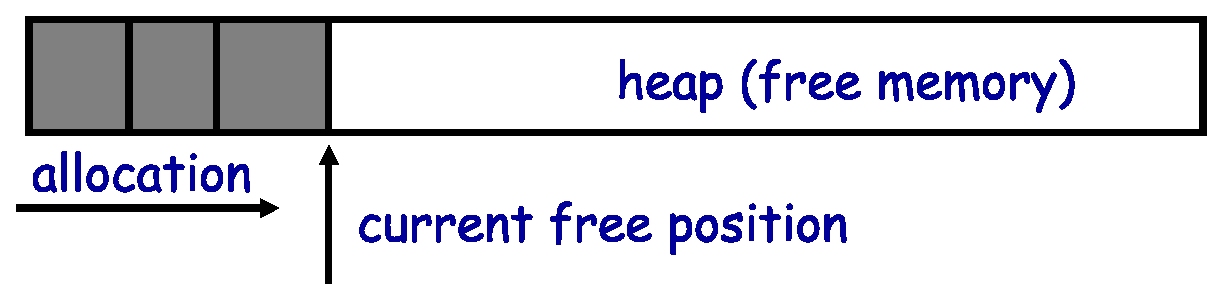
\includegraphics[width=4in]{figs/nofree}
  \item Problem: free creates holes (``fragmentation'')  Result?  Lots of free
space but cannot satisfy request! \\
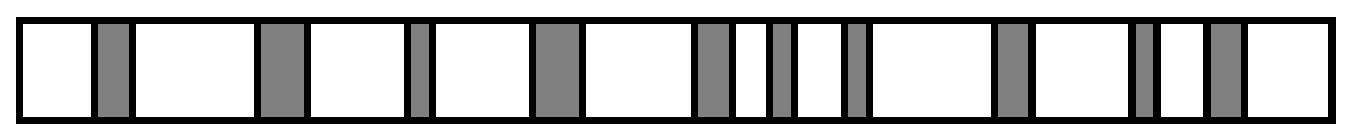
\includegraphics[width=4in]{figs/frag}

% Revive the tikz diagrams later
%\begin{tikzpicture}[node distance=-\pgflinewidth]
%\node[short,fill=gray!30] (a) {};
%\shnode{a}{b};
%\shnode{b}{c};
%\shnode{c}{d};
%\node[short,right=of d,fill=none,text width=8cm] (e) {Free Memory};
%\node[above right=0.5em of d] (ppre) {Current free pointer};
%\draw[->] (ppre.west) -- (d.north east);
%\draw[->] (a.north)+(0,0.5em) -- (d.north)+(0,0.5em);
%\end{tikzpicture}
}
\end{slide}

\begin{slide}{More abstractly}
\vspace{-1em}
\itms{
\item What an allocator must do:
\hbox to0pt{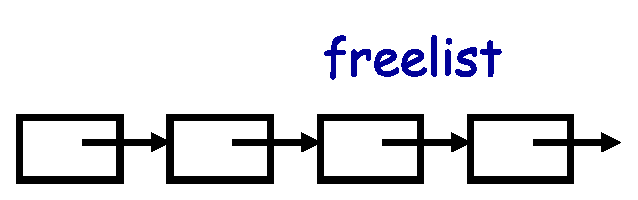
\includegraphics[width=2in]{figs/freelist}\hss}
\ittms{
  \item Track which parts of memory in use, which parts are free
  \item Ideal: no wasted space, no time overhead
}
\item What the allocator cannot do:
\ittms{
  \item Control order of the number and size of requested blocks
  \item Move allocated regions (bad placement decisions permanent)
}
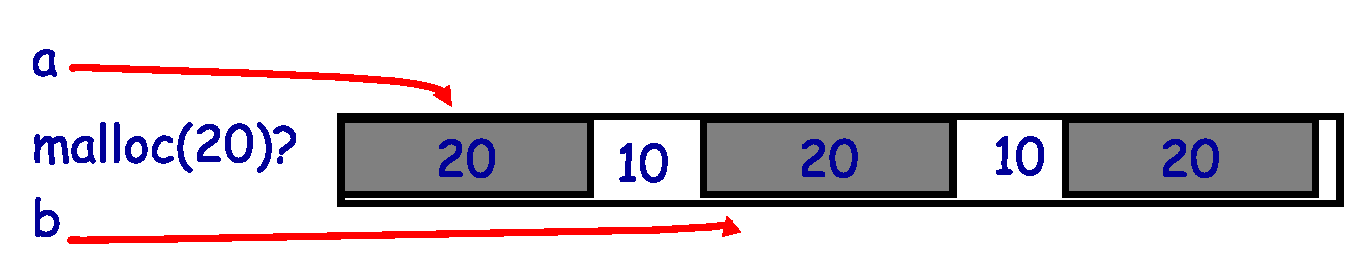
\includegraphics[width=4in]{figs/frag2}
\item The core fight: minimize fragmentation
\ittms{
  \item App frees blocks in any order, creating holes in ``heap''
  \item Holes too small? cannot satisfy future requests
}
} 
\end{slide}

\begin{slide}{What is fragmentation really?}
\itms{
\item Inability to use memory that is free
\item Two factors required for fragmentation
\ittms{
  \item Different lifetimes---if adjacent objects die at different
    times, then fragmentation:
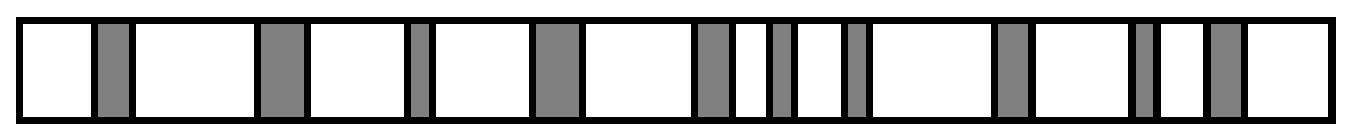
\includegraphics[width=4in]{figs/frags1}
    \begin{itemize}
      \item If they die at the same time, then no fragmentation:
    \end{itemize}
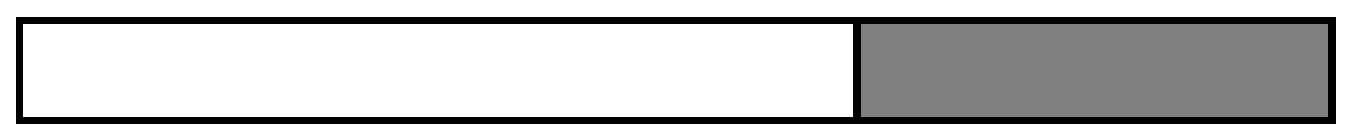
\includegraphics[width=4in]{figs/frags2}
  \item Different sizes: If all requests the same size, then no
    fragmentation \\
    (that's why no external fragmentation with paging):
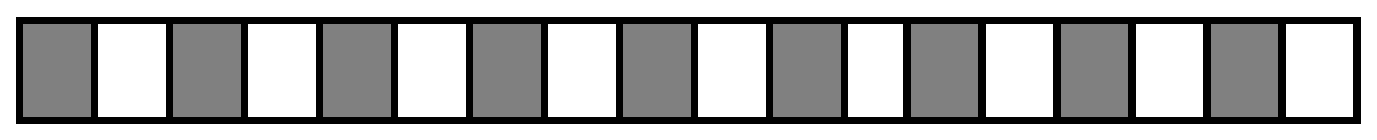
\includegraphics[width=4in]{figs/frags3}
}
}
\end{slide}

\begin{slide}{Important decisions}
\itms{
  \item Placement choice: where in free memory to put a requested block? 
\ittms{
    \item Freedom: can select any memory in the heap
    \item Ideal: put block where it won't cause fragmentation later
      (impossible in general: requires future knowledge)
}
  \item Split free blocks to satisfy smaller requests?
\ittms{
    \item Fights internal fragmentation
    \item Freedom: can choose any larger block to split
    \item One way: choose block with smallest remainder (best fit)
}
  \item Coalescing free blocks to yield larger blocks  \\
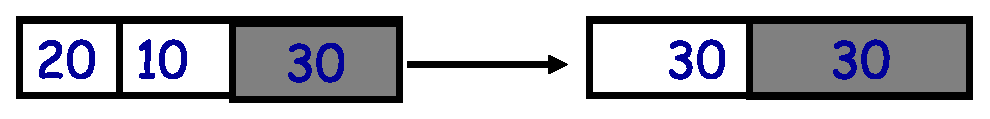
\includegraphics[width=3.5in]{figs/coalesce}
  \ittms{
    \item Freedom: when to coalesce (deferring can save work)
    \item Fights external fragmentation
  }
}
\end{slide}

\begin{slide}{Impossible to ``solve'' fragmentation}
\itms{
  \item If you read allocation papers to find the best allocator
  \ittms{
    \item All discussions revolve around tradeoffs
    \item The reason?  There cannot be a best allocator
  }
  \item Theoretical result: 
  \ittms{
    \item For any possible allocation algorithm, there exist streams of
      allocation and deallocation requests that defeat the allocator and
      force it into severe fragmentation.
  }
  \item How much fragmentation should we tolerate?
  \ittms{
    \item Let $M$~=~bytes of live data, $n_\mathrm{min}$~=~smallest
      allocation, $n_\mathrm{max}$~=~largest --
      How much gross memory required?
    \item Bad allocator: $M\cdot (n_\mathrm{max}/n_\mathrm{min})$ \\
      (only ever uses a memory location for a single size)
    \item Good allocator: $\sim M \cdot \log(n_\mathrm{max}/n_\mathrm{min})$
      %\href{http://portal.acm.org/citation.cfm?id=321658}{[Robson]}
% Allocate all M bytes in n_{min} size, then free every other one
% Repeat with remaining memory for next size, etc., up to n_{max}
  }
}
\end{slide}

\begin{slide}{Pathological examples}
\itms{
  \item Given allocation of 7 20-byte chunks \\
    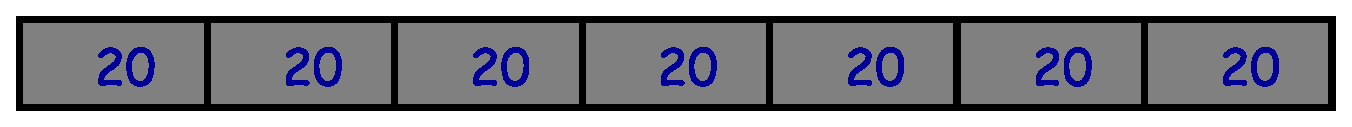
\includegraphics[width=4in]{figs/pathological1}
  \ittms{
    \item What's a bad stream of frees and then allocates?
      \onslide<2->{ \item Free every other chunk, then alloc 21 bytes}
  }
  \item Given a 128-byte limit on malloced space
    %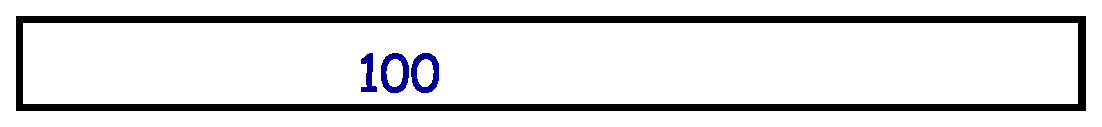
\includegraphics[width=4in]{figs/pathological2}
  \ittms{
    \item What's a really bad combination of mallocs \& frees?
      \onslide<3>{
        \item Malloc 128 1-byte chunks, free every other
        \item Malloc 32 2-byte chunks, free every other (1- \& 2-byte) chunk
        \item Malloc 16 4-byte chunks, free every other chunk\ldots
      }
  }
  \item Next: two allocators (best fit, first fit) that, in practice,
    work pretty well
  \ittms{
    \item ``pretty well'' = $\sim$20\% fragmentation under many workloads
  }
}
\end{slide}

\begin{slide}{Best fit}
\itms{
\item Strategy: minimize fragmentation by allocating space from block that leaves smallest fragment
\ittms{
  \item Data structure: heap is a list of free blocks, each has a
    header holding block size and pointers to next \\
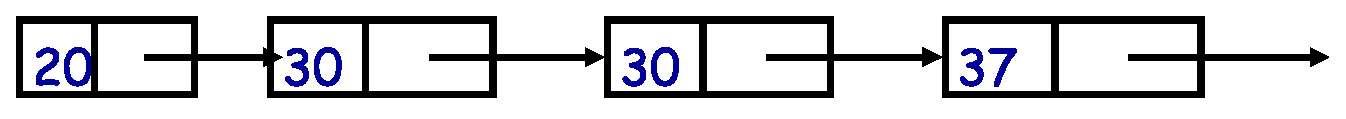
\includegraphics[width=4in]{figs/bestfit}
  \item Code: Search freelist for block closest in size to the
    request.  (Exact match is ideal) 
  \item During free (usually) coalesce adjacent blocks
}
\item Problem: Sawdust
\ittms{
  \item Remainder so small that over time left with ``sawdust'' everywhere
  \item Fortunately not a problem in practice
}
}
\end{slide}

\begin{slide}{Best fit gone wrong}
\itms{
  \item Simple bad case: allocate $n$, $m$ $(n<m)$ in alternating
    orders, free all the $n$s, then try to allocate an $n+1$
  \item Example: start with 100 bytes of memory
  \ittms{
    \item alloc 19, 21, 19, 21, 19 \\
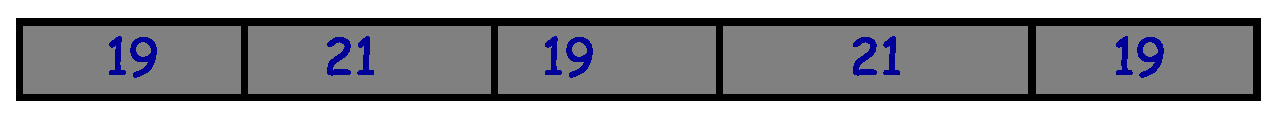
\includegraphics[width=4in]{figs/bestwrong1}
    \item free 19, 19, 19: \\
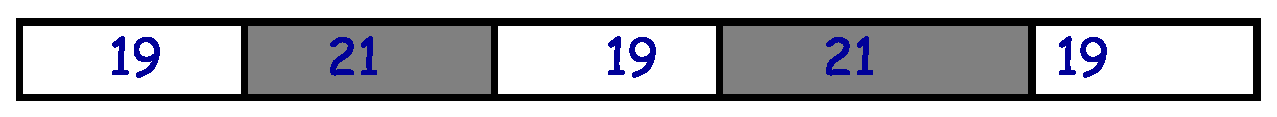
\includegraphics[width=4in]{figs/bestwrong2}
    \item alloc 20?  Fails!  (wasted space = 57 bytes)
  }
  \item However, doesn't seem to happen in practice (though the way
    real programs behave suggest it easily could)
}
\end{slide}

\begin{slide}{First fit}
\itms{
  \item Strategy: pick the first block that fits
  \ittms{
    \item Data structure: free list, sorted lifo, fifo, or by address
    \item Code: scan list, take the first one
   }
  \item LIFO: put free object on front of list. 
  \ittms{
    \item Simple, but causes higher fragmentation
    \item Potentially good for cache locality
  }
  \item Address sort: order free blocks by address
\ittms{
    \item Makes coalescing easy (just check if next block is free)
    \item Also preserves empty/idle space (locality good when paging)
}
  \item FIFO: put free object at end of list
\ittms{
    \item Gives similar fragmentation as address sort, but unclear why
}
}
\end{slide}

\begin{slide}{Subtle pathology:  LIFO FF}
\itms{
  \item Storage management example of subtle impact of simple decisions
  \item LIFO first fit seems good:
  \ittms{
    \item Put object on front of list (cheap), hope same size used
      again (cheap + good locality)
  }
  \item But, has big problems for simple allocation patterns:
  \ittms{
    \item E.g., repeatedly intermix short-lived $2n$-byte allocations,
      with long-lived $(n+1)$-byte allocations
    \item Each time large object freed, a small chunk will be quickly
      taken, leaving useless fragment.  Pathological fragmentation
%    \item In general, can easily build up lots of small fragments at
%      head of list -- increases search time
  }
}
\end{slide}

\begin{slide}{First fit: Nuances}
\itms{
\item First fit sorted by address order, in practice:
\ittms{
  \item Blocks at front preferentially split, ones at back only split when no larger one found before them
  \item Result? Seems to roughly sort free list by size 
  \item So? Makes first fit operationally similar to best fit: a first fit of a sorted list = best fit!
}
\item Problem: sawdust at beginning of the list
\ittms{
  \item Sorting of list forces a large requests to skip over many small blocks.  Need to use a scalable heap organization
}
\vspace*{-.05in}
  \item Suppose memory has free blocks:
\lower1ex\hbox to0pt{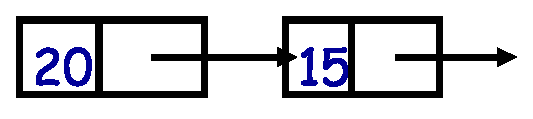
\includegraphics[width=1.7in]{figs/ffnuance}\hss}
\ittms{
  \item If allocation ops are 10 then 20, best fit wins
  \item When is FF better than best fit?
\pause
  \item Suppose allocation ops are 8, 12, then 12
           $\Longrightarrow$ first fit wins
}
}
\end{slide}

%% \begin{slide}{First/best fit: weird parallels}
%% \itms{
%%   \item Both seem to perform roughly equivalently
%%   \item In fact the placement decisions of both are roughly identical under both randomized and real workloads!
%%   \ittms{
%%     \item No one knows why
%%     \item Pretty strange since they seem pretty different
%%   }
%%   \item Possible explanations:
%%   \ittms{
%%     \item First fit like best fit because over time its free list
%%       becomes sorted by size: the beginning of the free list
%%       accumulates small objects and so fits tend to be close to best
%%     \item Both have implicit ``open space hueristic'' try not to cut
%%       into large open spaces: large blocks at end only used when have
%%       to be (e.g., first fit: skips over all smaller blocks)
%%   }
%% }
%% \end{slide}

\begin{slide}{Some worse ideas}
\itms{
\item Worst-fit: 
\ittms{
  \item Strategy: fight against sawdust by splitting blocks to
    maximize leftover size
  \item In real life seems to ensure that no large blocks around
  }
\item Next fit:
  \ittms{
  \item Strategy: use first fit, but remember where we found the last thing and start searching from there
  \item Seems like a good idea, but tends to break down entire list
}
\item Buddy systems:
\ittms{
  \item Round up allocations to power of 2 to make management faster
  \item Result? Heavy internal fragmentation
}
}
\end{slide}

\section{Exploiting program behavior}

\begin{slide}{Known patterns of real programs}
\itms{
\item So far we've treated programs as black boxes. 
\item Most real programs exhibit 1 or 2 (or all 3) of the following patterns
of alloc/dealloc:
\ittms{
  \item \emph{Ramps}: accumulate data monotonically over time \\
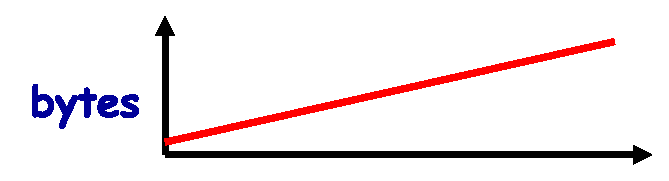
\includegraphics[width=2.2in]{figs/ramps}
  \item \emph{Peaks}: allocate many objects, use briefly, then free all \\
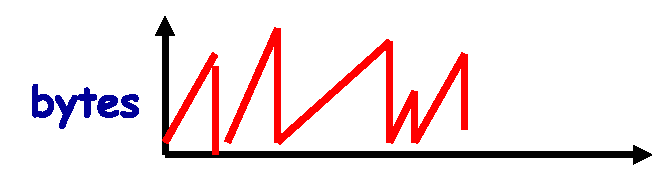
\includegraphics[width=2.2in]{figs/peaks}
  \item \emph{Plateaus}: allocate many objects, use for a long time \\
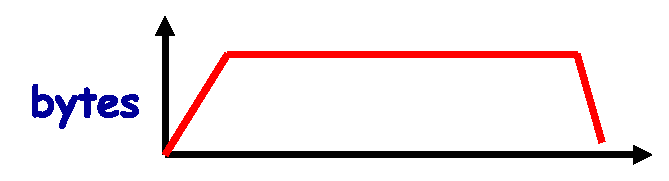
\includegraphics[width=2.2in]{figs/plateaus}
}
}
\end{slide}

\begin{slide}{Pattern 1: ramps}
\centerline{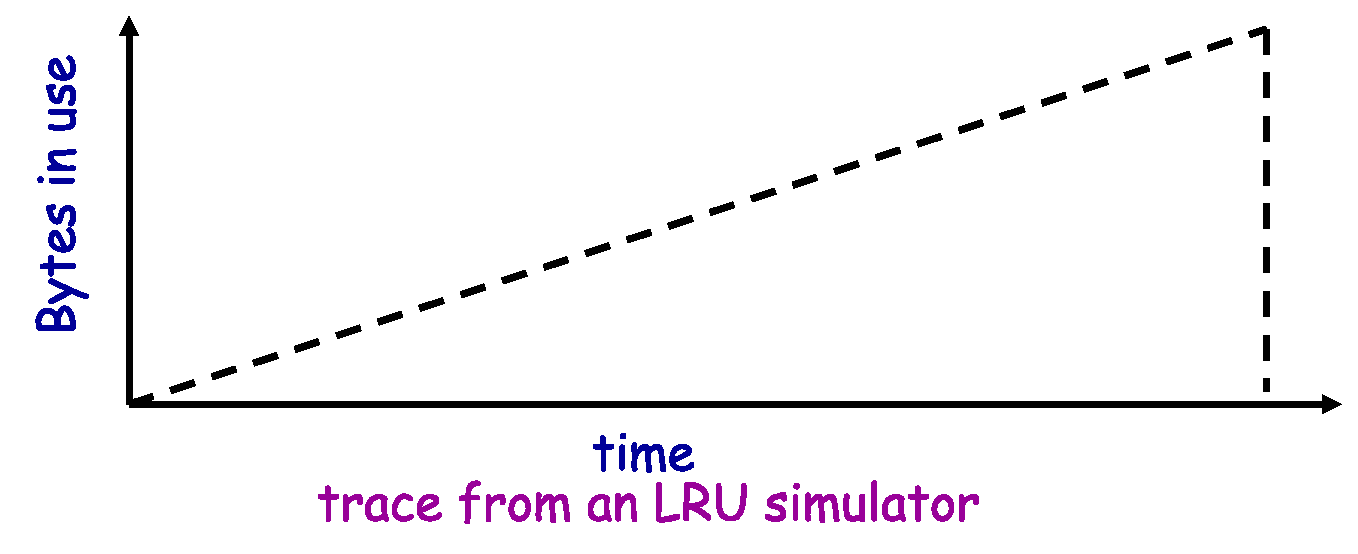
\includegraphics[width=4in]{figs/ramps-trace}}

\bigskip

\itms{
\item In a practical sense:  ramp = no free!
\ittms{
  \item Implication for fragmentation?
  \item What happens if you evaluate allocator with ramp programs only?
}
}
\end{slide}

\begin{slide}{Pattern 2: peaks}

\centerline{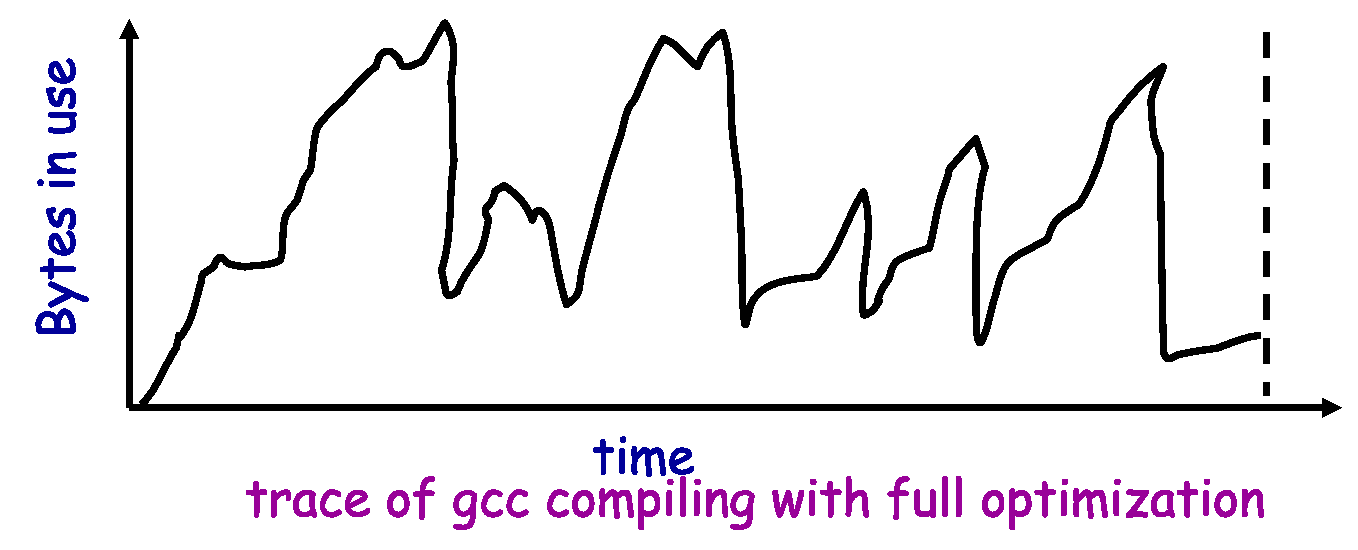
\includegraphics[width=4in]{figs/peaks-trace}}

\bigskip
\itms{
\item Peaks: allocate many objects, use briefly, then free all
\ittms{
  \item Fragmentation a real danger
  \item What happens if peak allocated from contiguous memory? 
  \item Interleave peak \& ramp? Interleave two different peaks? 
}
}
\end{slide}

\begin{slide}{Exploiting peaks}
\itms{
\item Peak phases: alloc a lot, then free everything
\ittms{
  \item So have new allocation interface: alloc as before, but only
    support free of everything
  \item Called ``arena allocation'', ``obstack'' (object stack), or
    \texttt{alloca}/procedure call (by compiler people)
}
\item Arena = a linked list of large chunks of memory
\ittms{
  \item Advantages: alloc is a pointer increment, free is ``free'' \\
    No wasted space for tags or list pointers \\[.1in]
  \centerline{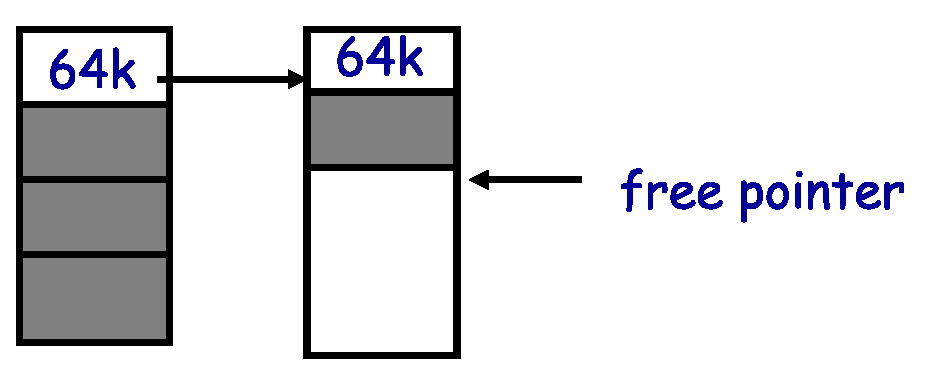
\includegraphics[height=1.15in]{figs/arena}}
}
}
\end{slide}

\begin{slide}{Pattern 3: Plateaus}
\centerline{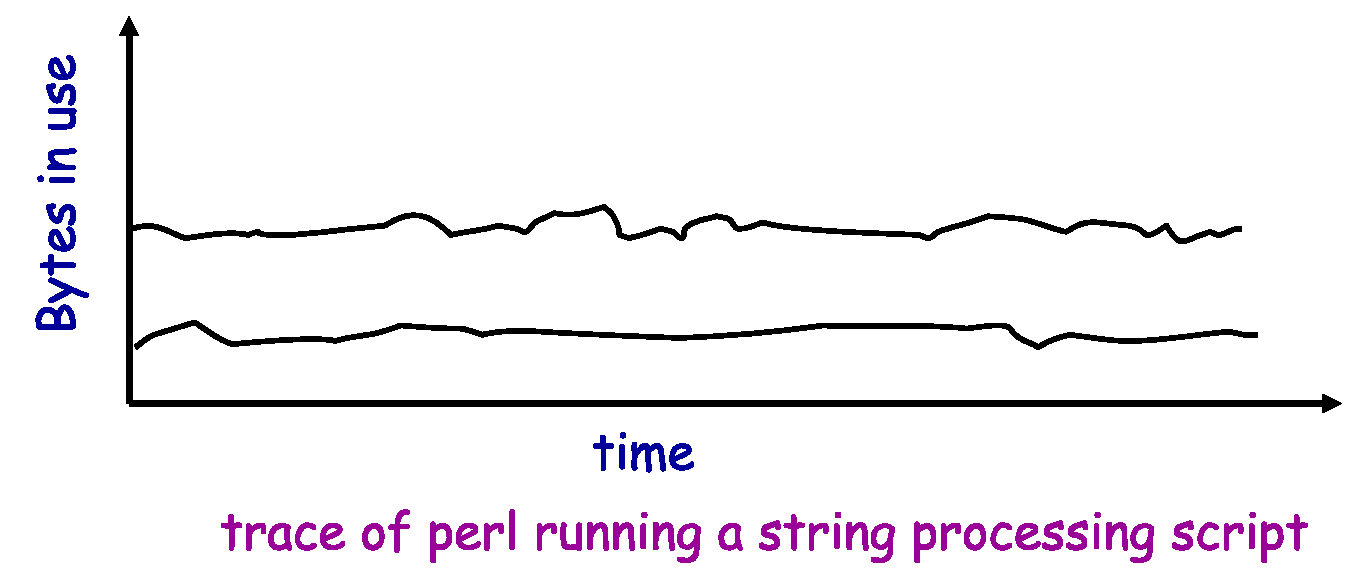
\includegraphics[width=4in]{figs/plateaus-trace}}

\bigskip

\itms{
  \item Plateaus: allocate many objects, use for a long time
  \ittms{
    \item What happens if overlap with peak or different plateau?
  }
}
\end{slide}

\begin{slide}{Fighting fragmentation}
\itms{
\item Segregation = reduced fragmentation:
\ittms{
  \item Allocated at same time $\sim$ freed at same time
  \item Different type $\sim$ freed at different time
}
\item[] 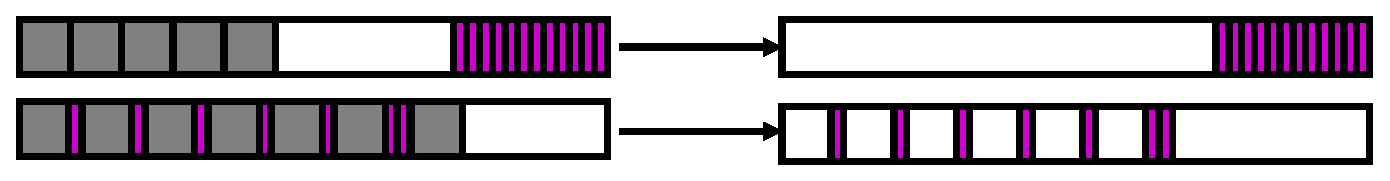
\includegraphics[width=4in]{figs/fightfrag}
\item Implementation observations:
\ittms{
  \item Programs allocate small number of different sizes
  \item Fragmentation at peak use more important than at low
  \item Most allocations small ($<$ 10 words)
  \item Work done with allocated memory increases with size
  \item Implications?
}
}
\end{slide}

\section{Allocator designs}

\begin{slide}{Slab allocation
    \cref{sched/readings/bonwick:slab.pdf}{[Bonwick]}}
\itms{
  \item Kernel allocates many instances of same structures
  \ittms{
    \item E.g., a 1.7 KB \texttt{task\_struct} for every process on system
  }
  \item Often want contiguous \emph{physical} memory (for DMA)
  \item Slab allocation optimizes for this case:
  \ittms{
    \item A \Red{slab} is multiple pages of contiguous physical memory
    \item A \Red{cache} contains one or more slabs
    \item Each cache stores only one kind of object (fixed size)
  }
  \item Each slab is \Red{full}, \Red{empty}, or \Red{partial}
  \item E.g., need new \texttt{task\_struct}?
  \ittms{
    \item Look in the \texttt{task\_struct} cache
    \item If there is a partial slab, pick free \texttt{task\_struct} in that
    \item Else, use empty, or may need to allocate new slab for cache
  }
  \item Advantages:  speed, and no internal fragmentation
}
\end{slide}

\begin{slide}{Simple, fast segregated free lists}
\centerline{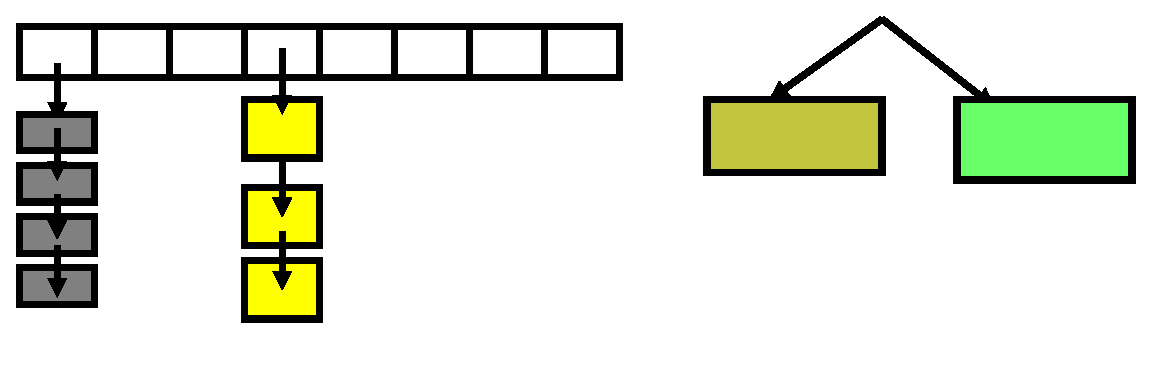
\includegraphics[width=4in]{figs/segregated-free}}

\medskip

\itms{
\item Array of free lists for small sizes, tree for larger
\ittms{
  \item Place blocks of same size on same page
  \item Have count of allocated blocks: if goes to zero, can return page
}
\item Pro: segregate sizes, no size tag, fast small alloc
\item Con: worst case waste: 1 page per size even w/o free,
  after pessimal free waste 1 page per object
  \item TCMalloc
    \href{http://goog-perftools.sourceforge.net/doc/tcmalloc.html}{[Ghemawat]}
    is a well-documented malloc like this
}
\end{slide}

\begin{slide}{Typical space overheads}
\itms{
  \item Free list bookkeeping + alignment determine minimum allocatable size:
  \ittms{
    \item Store size of block
    \item Pointers to next and previous freelist element
  }
  \item[] 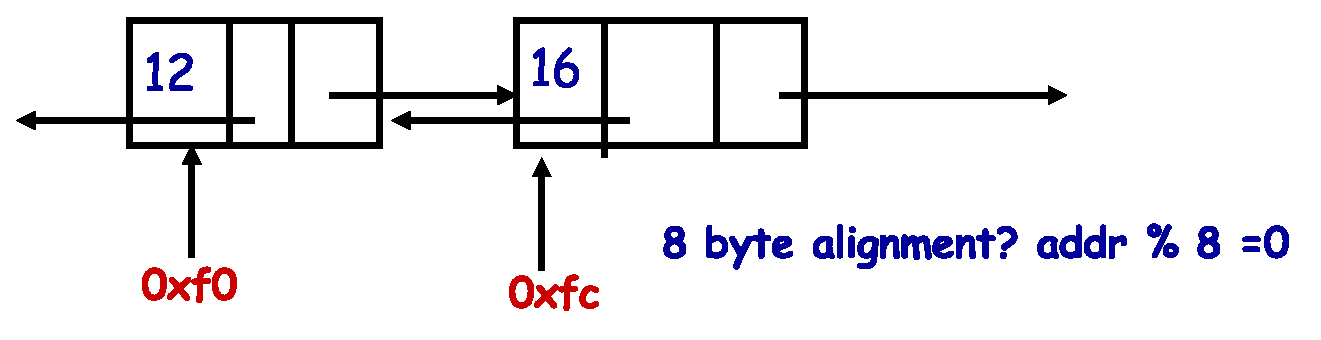
\includegraphics[width=4in]{figs/overhead}
  \ittms{
    \item Machine enforced overhead: alignment.  Allocator doesn't
      know type.  Must align memory to conservative boundary
    \item Minimum allocation unit?  Space overhead when allocated?
  }
}
\end{slide}

\begin{slide}{Getting more space from OS}
\itms{
  \item On Unix, can use \texttt{sbrk}
  \ittms{
  \item  E.g., to activate a new zero-filled page: \\
     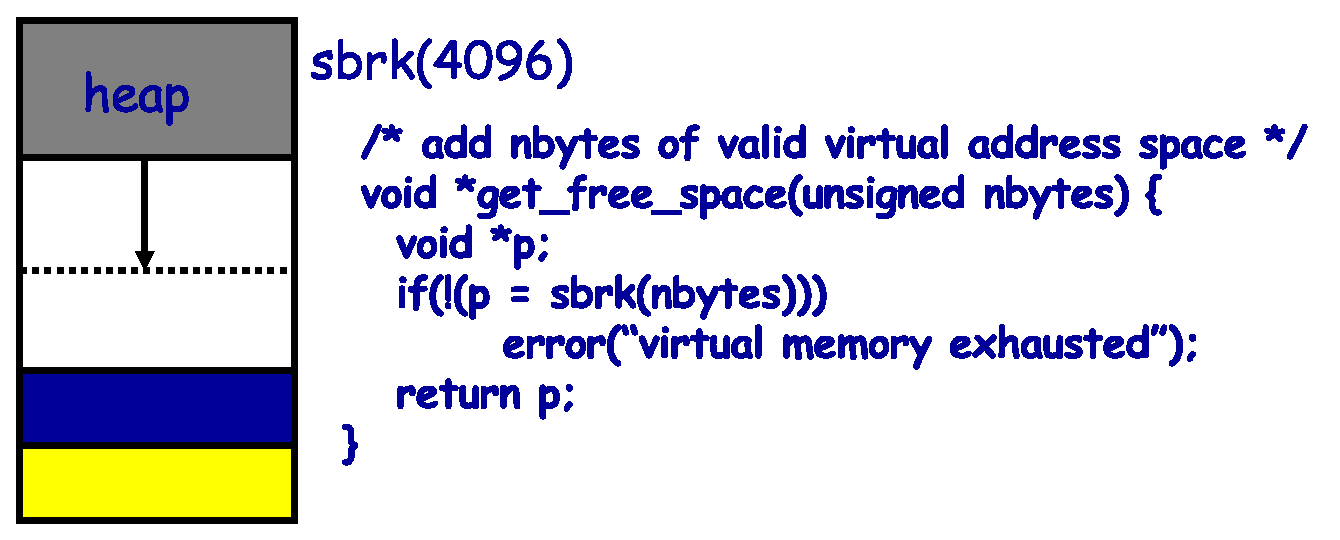
\includegraphics[height=1.5in]{figs/sbrk}
  }
  \item For large allocations, \texttt{sbrk} a bad idea
  \ittms{
    \item May want to give memory back to OS
    \item Can't with \texttt{sbrk} unless big chunk last thing
      allocated
    \item So allocate large chunk using \texttt{mmap}'s
      \texttt{MAP\_ANON}
  }
}
\end{slide}

%\section{User-level MMU tricks}
%
%\begin{slide}{Faults + resumption = power}
%\itms{
%\item Resuming after fault lets us emulate many things
%\ittms{
%  \item ``every problem can be solved with layer of indirection''
%}
%\item Example: sub-page protection
%\item To protect sub-page region in paging system:
%\ittms{
%  \item[] \hspace*{.07in} 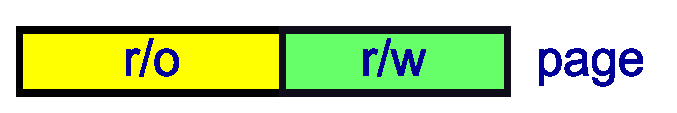
\includegraphics[height=.3in]{figs/resume1}
%  \item  Set entire page to weakest permission; record in PT \\
%  \centerline{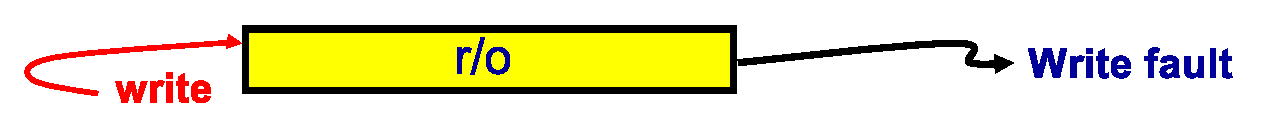
\includegraphics[height=.4in]{figs/resume2}}
%  \item Any access that violates perm will cause an access fault  
%  \item Fault handler checks if page special, and if so, if access allowed. Continue or raise error, as appropriate
%}
%}
%\end{slide}
%
%\begin{slide}{More fault resumption examples}
%\itms{
%\item Emulate accessed bits:
%\ittms{
%  \item Set page permissions to ``invalid''.  
%  \item On any access will get a fault: Mark as accessed
%}
%\item Avoid save/restore of FP registers
%\ittms{
%  \item Make first FP operation fault to detect usage
%}
%\item Emulate non-existent instructions:
%\ittms{
%  \item Give inst an illegal opcode; OS fault handler detects and
%    emulates fake instruction
%}
%}
%\vspace*{-.1in}
%\hbox{\hspace*{-.03in}
%\begin{minipage}{3.1in}
%\itms{
%\item Run OS on top of another OS! 
%\ittms{
%  \item Slam OS into normal process
%  \item When does something ``privileged,''
%    real OS gets woken up with a fault. 
%  \item If op allowed, do it, otherwise kill. 
%  \item IBM's VM/370. Vmware (sort of)
%}
%}
%\end{minipage}
%\begin{minipage}{1.5in}
%\vspace{1em}
%  \centerline{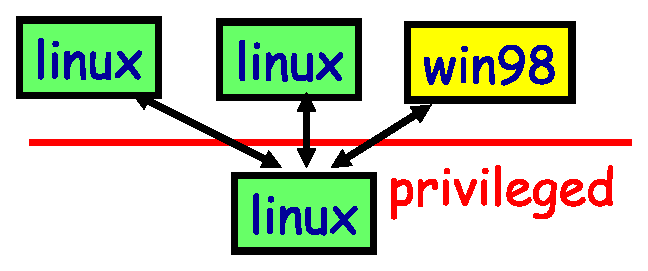
\includegraphics[width=48mm]{figs/vm}}
%\vbox to.8 in{\vss}
%\end{minipage}
%}
%\end{slide}
%
%\begin{slide}{Not just for kernels}
%\itms{
%  \item User-level code can resume after faults, too
%  \item \texttt{mprotect} -- protects memory
%  \item \texttt{sigaction} -- catches signal after page fault
%  \ittms{
%    \item Return from signal handler restarts faulting instruction
%  }
%  \item Many applications detailed by
%    \cref{sched/readings/vmpup.pdf}{[Appel \& Li]}
%  \item Example:  concurrent snapshotting of process
%  \ittms{
%    \item Mark all of process's memory read-only w.\ \texttt{mprotect}
%    \item One thread starts writing all of memory to disk
%    \item Other thread keeps executing
%    \item On fault -- write that page to disk, make writable, resume
%  }
%}
%\end{slide}
%
%\begin{slide}{Distributed shared memory}
%\centerline{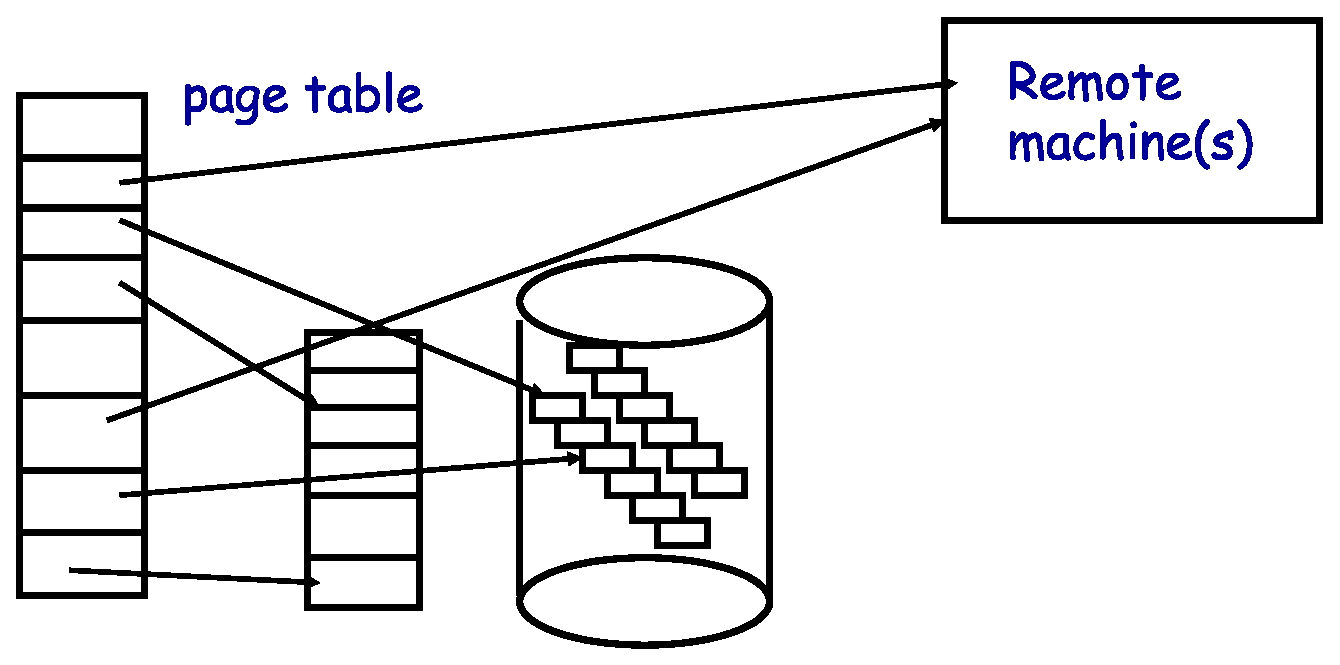
\includegraphics[height=2in]{figs/dsm}}
%\medskip
%\itms{
%  \item Virtual memory allows us to go to memory or disk
%  \ittms{
%    \item But, can use the same idea to go anywhere!  Even to another computer.
%         Page across network rather than to disk.  Faster, and allows network
%         of workstations (NOW)
%}
%}
%\end{slide}
%
%\begin{slide}{Persistent stores}
%\itms{
%  \item Idea:  Objects that persist across program invocations
%  \ittms{
%    \item E.g., object-oriented database; useful for CAD/CAM type apps
%  }
%  \item Achieve by memory-mapping a file
%  \item But only write changes to file at end if commit
%  \ittms{
%    \item Use dirty bits to detect which pages must be written out
%    \item Or emulate dirty bits with \emph{mprotect}/\emph{sigaction}
%      (using write faults)
%  }
%  \item On 32-bit machine, store can be larger than memory
%  \ittms{
%    \item But single run of program won't access $>$ 4GB of objects
%    \item Keep mapping betw.\ 32-bit mem ptrs and 64-bit disk offsets
%    \item Use faults to bring in pages from disk as necessary
%    \item After reading page, translate pointers---known as
%      \emph{swizzling}
%  }
%}
%\end{slide}

\section{Garbage collection}

\begin{slide}{Garbage collection}
\itms{
  \item In safe languages, run time knows about all pointers
  \ittms{
    \item So can move an object if you change all the pointers
  }
  \item What memory locations might a program access?
  \ittms{
    \item Any objects whose pointers are currently in registers
    \item Recursively, any pointers in objects it might access
    \item Anything else is \emph{unreachable}, or \emph{garbage};
      memory can be re-used
  }
  \item Example: stop-and-copy garbage collection
  \ittms{
    \item Memory full?  Temporarily pause program, allocate new heap
    \item Copy all objects pointed to by registers into new heap
    \ittms{
      \item Mark old copied objects as copied, record new location
    }
    \item Start scanning through new heap.  For each pointer:
    \ittms{
      \item Copied already?  Adjust pointer to new location
      \item Not copied?  Then copy it and adjust pointer
    }
    \item Free old heap---program will never access it---and continue
  }
}
\end{slide}

\begin{slide}{Concurrent garbage collection}
\itms{
  \item Idea:  Stop \& copy, but without the stop
  \ittms{
    \item \emph{Mutator} thread runs program, \emph{collector}
      concurrently does GC
  }
  \item When collector invoked:
  \ittms{
    \item Protect from space \& unscanned to space from mutator
    \item Copy objects in registers into \emph{to space}, resume mutator
    \item All pointers in scanned \emph{to space} point to \emph{to space}
    \item If mutator accesses unscanned area, fault, scan page, resume
  }
}
\centerline{\input{baker}}
\centerline{(See \cref{readings/vmpup.pdf}{[Appel \& Li]}.)}
\end{slide}

\begin{slide}{Heap overflow detection}
\itms{
  \item Many GCed languages need fast allocation
  \ittms{
    \item E.g., in lisp, constantly allocating cons cells
    \item Allocation can be as often as every 50 instructions
  }
  \item Fast allocation is just to bump a pointer
}
\begin{ccode}
        char *next_free;
        char *heap_limit;

        void *alloc (unsigned size) {
          if (next_free + size > heap_limit)     /* 1 */
            invoke_garbage_collector ();         /* 2 */
          char *ret = next_free;
          next_free += size;
          return ret;
        }       
\end{ccode}
\itms{
  \item But would be even faster to eliminate lines 1 \& 2!
}
\end{slide}

\begin{slide}{Heap overflow detection 2}
\itms{
  \item Mark page at end of heap inaccessible
  \ittms{
    \item \texttt{mprotect (heap\_limit, PAGE\_SIZE, PROT\_NONE);}
  }
  \item Program will allocate memory beyond end of heap
  \item Program will use memory and fault
  \ittms{
    \item Note:  Depends on specifics of language
    \item But many languages will touch allocated memory immediately
  }
  \item Invoke garbage collector
  \ittms{
    \item Must now put just allocated object into new heap
  }
  \item Note:  requires more than just resumption
  \ittms{
    \item Faulting instruction must be resumed
    \item But must resume with different target virtual address
    \item Doable on most architectures since GC updates registers
  }
}
\end{slide}

\begin{slide}{Reference counting}
\vspace{-1em}
\begin{minipage}{3.4in}
\itms{
  \item Seemingly simpler GC scheme:
  \ittms{
    \item Each object has ``ref count'' of pointers to it
    \item Increment when pointer set to it
    \item Decremented when pointer killed
      (C++ destructors handy for such ``smart pointers'')
  }
}
\end{minipage}
\begin{minipage}{.8in}
\centerline{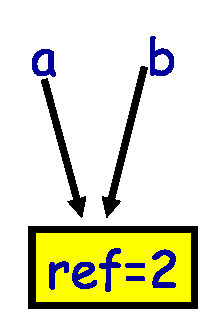
\includegraphics[width=.8in]{figs/refcnt1}}
\end{minipage}
\vspace*{-\baselineskip}
\itms{
  \item[]
  \ittms{
    \item[] 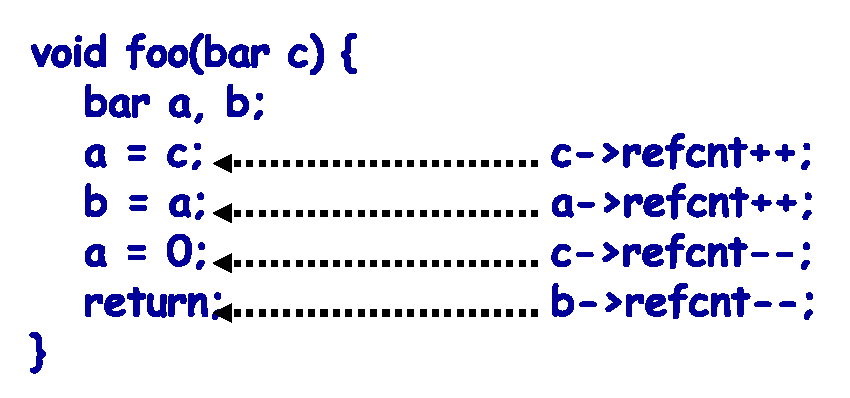
\includegraphics[height=1.3in]{figs/refcnt2}
    \item ref count == 0?  Free object
  }
  \item Works well for hierarchical data structures
  \ittms{
    \item E.g., pages of physical memory
  }
}
\end{slide}

\begin{slide}{Reference counting pros/cons}
\vspace{-1em}
\itms{
  \item Circular data structures always have ref count $>$ 0
  \ittms{
    \item No external pointers means \Red{lost memory} \\
        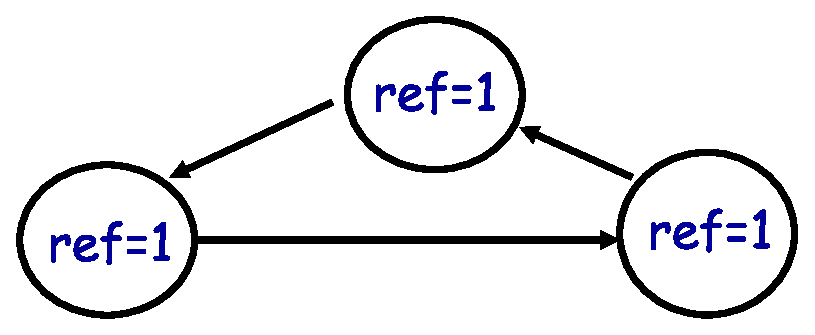
\includegraphics[width=2.7in]{figs/cycle}
  }
  \item Can do manually w/o PL support, but error-prone
  \item Potentially more efficient than real GC
  \ittms{
    \item No need to halt program to run collector
    \item Avoids weird unpredictable latencies
  }
  \item Potentially less efficient than real GC
  \ittms{
    \item With real GC, copying a pointer is cheap
    \item With reference counting, must write ref count each time
  }
}
\end{slide}

\end{document}

% Local Variables:
% tex-command: "gmake;:"
% tex-dvi-view-command: "gmake preview;:"
% End:

